\PassOptionsToPackage{dvipsnames,table}{xcolor}
\documentclass[11pt,a4paper]{article}

\usepackage{Act}

\begin{document}
\input{\detokenize{/home/fenarius/Travail/Cours/cpge-info/latex/Macros.tex}}
\ModeExercice
\TPnote{2}{Langage C}

%Nom de la première activité
\setcounter{Exercise}{0}


\begin{Exercise}[title={Code de César}]

	L'une des plus ancienne méthodes de chiffrement est le code de César qui consiste simplement à décaler chaque lettre d'une distance fixe dans l'alphabet. Par exemple si cette distance (appelée clé de chiffrement) est 3, la lettre $A$ devient $D$, $B$ devient $E$, et ainsi de suite. Pour les dernières lettres on reprend au début de l'alphabet. Par exemple toujours avec une distance de 3, $X$ devient $A$, $Y$ devient $B$ et $Z$ devient $C$. Ce fonctionnement est illustré ci-dessous : \medskip
	\begin{center}
		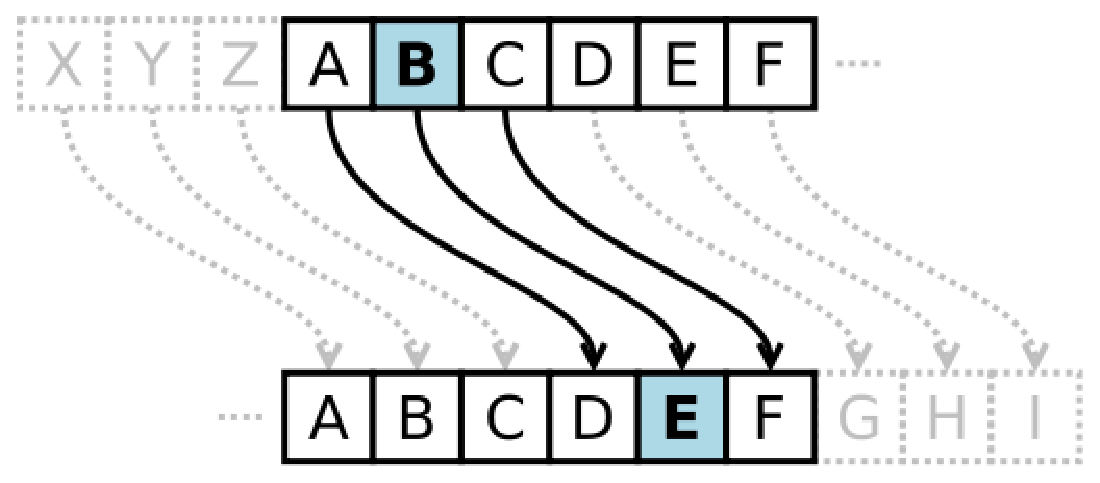
\includegraphics[width=8cm]{cesar.eps}
	\end{center}

	Le but de l'exercice est de créer un exécutable {\tt cesar.exe} qui prend en argument une chaine de caractères et une clé de chiffrement et affiche le texte chiffré correspondant. On ne décalera que les lettres (majuscules ou mininuscules) et on laissera les autres caractères intacts. Par exemple :
	\begin{mdframed}
		\begin{verbatim}
./cesar.exe "La MP2I c'est trop bien !" 7
Sh TW2P j'lza ayvw iplu !
./cesar.exe "Sh TW2P j'lza ayvw iplu !" -7
La MP2I c'est trop bien !
\end{verbatim}
	\end{mdframed}
	\aide \; On rappelle qu'en C, un caractère est represénté par son code {\sc ascii} et donc une comparaison comme {\tt car >= 'A'} où {\tt car} est de type {\tt char} est tout a fait légitime car on compare en fait les codes {\sc ascii}.
	\Question{Ecrire une fonction {\tt chiffre\_caractere} qui prend en argument un caractère  {\tt car}  et un entier {\tt cle} et renvoie un le caractère {\tt car} chiffré avec le décalage {\tt cle} tel que décrit ci-dessus.\\ Par exemple {\tt chiffre\_caractere('A',3)} doit renvoyer {\tt 'D'}. On rappelle qu'on laisse intact les caractères autres que les lettres majuscules ou minuscules, donc par exemple {\tt chiffre\_caractere('!',3)} renvoie {\tt '!'}. \\
	\aide \; En cas de difficultés sur cette première question, pour ne pas rester bloqué, poursuivre l'exercice en utilisant à la place une fonction qui renvoie simplement le caractère passé en argument.}
    \inputpartC{cesar.c}{}{}{5}{21}
	\Question{Ecrire une fonction {\tt chiffre\_chaine} qui prend en argument une chaine de caractères et et un entier {\tt cle} et renvoie la chaine chiffrée avec le code de César de décalage {\tt cle}. \\
	\danger \; On rappelle qu'en C, une chaine de caractères est un tableau de caractères équipé d'une sentinelle marquant la fin de la chaine. Ainsi la chaine {\tt "MP2I"} est de longueur 4 mais occupe 5 caractères en mémoire (le dernier est {\tt '\textbackslash{}0'}).
    \inputpartC{cesar.c}{}{}{23}{33}
	\Question{Ecrire une fonction {\tt main} qui  prend deux arguments en ligne de commande (la chaine à chiffrer et la clé) et affiche la chaine chiffrée dans le terminal. Si on donne à l'exécutable moins de deux arguments, un message d'erreur s'affiche.
		Par exemple :
		\begin{mdframed}
			\begin{verbatim}
./cesar.exe "Hello" 11
Spwwz
./cesar.exe "Trop cool"
Erreur, il faut donner une chaine et une clé de chiffrement
\end{verbatim}
		\end{mdframed}
	}
	\aide \; On rappelle que l'entier fourni en ligne de commande est une chaine de caractères et que pour le convertir en {\tt int}, on utilise la fonction {\tt atoi} disponible dans {\tt <stdlib.h>}
	}
    \inputpartC{cesar.c}{}{}{35}{48}
	\Question{Ecrire un nouvel executable {\tt cesar\_fichier} qui prend en argument un nom de fichier (à la place de la chaine de caractères) ainsi qu'un entier {\tt cle}. C'est le contenu du fichier (limité à 255 caractères) qui est alors chiffré avec le decalage {\tt cle} donné, le résultat est écrit dans le terminal comme précédemment.\\
		\aide \; On pourra utiliser la fonction {\tt fgetc} qui lit un caractère sur le flux de lecture donné en argument.}
    \inputpartC{cesar_fichier.c}{}{}{35}{59}
\end{Exercise}


\end{document}
